\documentclass[12pt,a4paper,openright,twoside]{report}
% chktex-file 1 % Ignora i warning di spazio dopo i comandi

% ====================================================
%
% PACCHETTI
%
% ====================================================
\usepackage[italian]{babel}
\usepackage[utf8]{inputenc}
\usepackage{graphicx}
\usepackage{fancyhdr}
\usepackage{indentfirst}
\usepackage{float}
\usepackage{amssymb, amsmath, latexsym, amsthm, gensymb}
\usepackage[a4paper]{geometry}
\usepackage[pdfpagelabels]{hyperref}
\usepackage[italian, capitalise]{cleveref}
\crefname{figure}{Figura}{Figure}
\Crefname{figure}{Figura}{Figure}
\usepackage{caption}
\usepackage{subcaption}
\usepackage{emptypage} % Permette di usare \cleardoublepage invece di \clearpage{\pagestyle{empty}\cleardoublepage}
\usepackage[bottom]{footmisc} % Forza la nota a piè di pagina a essere in fondo alla pagina
\usepackage{lineno}
\usepackage{needspace}

% ====================================================
%
% CONFIGURAZIONI
%
% ====================================================
\graphicspath{ {./resources/img/} }
\linespread{1.3}
\raggedbottom{} % Non forzare il contenuto a riempire la pagina
\setlength{\intextsep}{20pt}   % Spazio sopra e sotto le figure posizionate con [h] o [H]

% Configurazione Intestazioni
\pagestyle{fancy}
\renewcommand{\chaptermark}[1]{\markboth{\thechapter.\ #1}{}}
\renewcommand{\sectionmark}[1]{\markright{\thesection{} \ #1}{}}
\rhead[\fancyplain{}{\bfseries\leftmark}]{\fancyplain{}{\bfseries\thepage}}
\lhead[\fancyplain{}{\bfseries\thepage}]{\fancyplain{}{\bfseries\rightmark}}
\cfoot{}

\begin{document}

% ====================================================
%
% FRONTESPIZIO
%
% ====================================================
\begin{titlepage}
% Forziamo margini simmetrici e textwidth a 450pt per il frontespizio
\newgeometry{left=75pt, right=75pt, top=2cm, bottom=2.5cm}
% OLD: \newgeometry{left=72pt, right=72pt, top=2cm, bottom=2cm}
\setlength{\textwidth}{450pt}

\begin{center}
    
\includegraphics[width=0.25\linewidth]{logo_unibo.png}\vspace{0.7cm}\\

    {{\Large{\textsc{Alma Mater Studiorum $\cdot$ Universit\`a di Bologna}}}} \\
    \rule[0.1cm]{15.8cm}{0.1mm}
    \rule[0.5cm]{15.8cm}{0.6mm}

    {\small{\bf DIPARTIMENTO DI INFORMATICA --- SCIENZA E INGEGNERIA\\
    Corso di Laurea in Ingegneria e Scienze Informatiche}}
\end{center}

\vfill

\begin{center}
    {\LARGE{\bf
        \linespread{1}\selectfont
        Progettazione e sviluppo di un Event Display 3D interattivo basato su OpenGL per il rivelatore SND@LHC\par
    }}
    \vspace{19mm}
    {\large{\bf Tesi di Laurea in Computer Graphics}}
\end{center}

\vfill

\par
\noindent
\begin{minipage}[t]{0.50\textwidth}
    {\large{\bf Relatrice:\\[1mm]
    Prof.ssa Damiana Lazzaro}} \\[8mm]
    {\large{\bf Correlatori: \\[1mm]
    Prof. Luigi Guiducci \\
    Dott.ssa Giulia Paggi}}
\end{minipage}
\hfill
\begin{minipage}[t]{0.47\textwidth}\raggedleft{}
    {\large{\bf Presentata da:\\[1mm]
    Enrico Bartocetti}}
\end{minipage}

\vfill

\begin{center}
    {\large{\bf Sessione Unica\\}}
    {\large{\bf Anno Accademico 2025/2026}}
\end{center}
\end{titlepage}


% ====================================================
%
% CAMBIAMENTO GEOMETRIA PER IL RESTO DELLA TESI
%
% ====================================================
\restoregeometry

% Margini classici: 3.5cm sopra/sotto e 3cm ai lati + rilegatura
\newgeometry{
    lines=34,
    includehead,
    vmarginratio=1:1, % Centra verticalmente il blocco delle 33 righe
    bindingoffset=7mm, % Spazio per la rilegatura
    inner=35mm,       % Margine interno (lato rilegatura)
    outer=40mm        % Margine esterno
}
%Per la riga di intestazione
\setlength{\headwidth}{\textwidth}
\addtolength{\headwidth}{20pt} % Circa 7 mm

% Vecchia gestione margini alterni:
% \setlength{\oddsidemargin}{30pt}
% \setlength{\evensidemargin}{20pt}


% ====================================================
%
% DEDICA, INDICI E INTRO
%
% ====================================================
\cleardoublepage
\thispagestyle{empty}
\vspace*{6.5cm}
\begin{flushright}
    \large \em
    Questa è la \textsc{Dedica}.
\end{flushright}

\cleardoublepage
\pagenumbering{roman}
\tableofcontents % Indice

\cleardoublepage
\phantomsection
\addcontentsline{toc}{chapter}{Elenco delle Figure}
\listoffigures % Indice delle figure

\cleardoublepage
\linenumbers
\chapter*{Introduzione}
\addcontentsline{toc}{chapter}{Introduzione}
\markboth{Introduzione}{}
SND@LHC è un esperimento di fisica delle particelle situato al CERN, che ha come obiettivo lo studio delle interazioni dei neutrini in un intervallo di energie precedentemente inesplorato.
Lo studio di queste particelle offre infatti una nuova chiave di lettura su fenomeni che vanno oltre il Modello Standard, la teoria attualmente alla base della fisica delle particelle.

La collaborazione di SND@LHC, tra i vari strumenti software a disposizione per la ricostruzione e lo studio degli eventi, utilizza un event display.
Un event display è un software grafico che permette di visualizzare i segnali letti dai sensori all'interno del rivelatore, così da ricostruire quanto accaduto.
Il software attuale è però affetto da alcune significative limitazioni.
Mette innanzitutto a disposizione solo due viste fisse, ovvero le proiezioni bidimensionali laterali e dall'alto del rivelatore, impedendo qualsiasi interazione con la geometria.
È inoltre affetto da gravi carenze di usabilità: il suo avvio richiede di utilizzare molti argomenti mnemonici da riga di comando, e il passaggio a un evento di una run diversa richiede il riavvio del software.
Infine, non prevede alcuna modularità, dato che l'intero software è contenuto in un unico file Python.

Con questa tesi si vuole realizzare un nuovo event display per la collaborazione, basato su una scena tridimensionale interattiva.
Il nuovo sistema dovrà inoltre offrire una buona usabilità e rispettare le pratiche di buona progettazione del software, così da garantirne la manutenibilità e l'estendibilità nel tempo.

Il lavoro inizia descrivendo dettagliatamente l'esperimento SND@LHC, a partire dalla sua collocazione fino al dettaglio di ogni sottorivelatore, proseguendo poi con lo studio del software attuale e un'analisi dei requisiti discussi con la collaborazione.
Successivamente verranno presentate le basi matematiche di computer grafica necessarie alla costruzione del motore di rendering tridimensionale, così da comprendere nel dettaglio ogni scelta implementativa.
Segue un capitolo che descrive l'architettura del software, basata su un ampio utilizzo di design pattern per ricondurre le principali sfide progettuali a problemi noti, con soluzioni consolidate.
La teoria e le scelte progettuali vengono poi applicate nella stesura del software, descritta in dettaglio in un apposito capitolo e accompagnata da porzioni rilevanti di codice commentato.
Vengono infine mostrate, tramite schermate dell'interfaccia utente, le funzionalità implementate nel software, così da illustrare concretamente come il nuovo event display possa migliorare lo studio degli eventi da parte della collaborazione di SND@LHC.
La tesi si chiude con un capitolo conclusivo, in cui vengono riassunti i risultati raggiunti, discussi i limiti del sistema sviluppato e proposti possibili sviluppi futuri.

% ====================================================
%
% CORPO DELLA TESI
%
% ====================================================
\cleardoublepage
\pagenumbering{arabic}
\chapter{L’esperimento SND@LHC}

SND@LHC (\textit{Scattering and Neutrino Detector at the LHC}) è un esperimento il cui obiettivo è lo studio di neutrini ad alta energia prodotti nel Large Hadron Collider.
Lo scattering (o diffusione / dispersione) è un fenomeno fisico in cui particelle o onde vengono deflesse e disperse in varie direzioni a causa dell'interazione con altre particelle o ostacoli.
SND@LHC è stato approvato nel 2021, costruito, installato e messo in funzione in circa un anno e ha iniziato a raccogliere dati durante la Run 3 dell'LHC, iniziata nel luglio 2022.

% ====================================================
%
% IL CERN E LHC
%
% ====================================================
\section{Il CERN e LHC}
Il CERN (Organizzazione Europea per la Ricerca Nucleare, in francese \textit{Conseil Européen pour la Recherche Nucléaire}) è il laboratorio di fisica delle particelle più grande al mondo, fondato il 29 settembre 1954.
Si trova al confine tra la Francia e la Svizzera, più precisamente alla periferia ovest della città di Ginevra, nel comune di Meyrin.

Ospita un ampio complesso di acceleratori di particelle, illustrato in \cref{fig:acceleratori_cern}.
Un acceleratore di particelle accelera particelle cariche, come protoni o elettroni, ad altissime velocità prossime a quella della luce: queste particelle vengono poi fatte collidere con un bersaglio o con altre particelle che circolano nella direzione opposta.
L'energia liberata si trasforma poi in materia sottoforma di altre particelle (le più massicce delle quali dominavano l'universo primordiale), seguendo la famosa equazione di Einstein $E = mc^2$ \cite{CERN_Acceleratori}.

\begin{figure}[H]
	\centering{}
	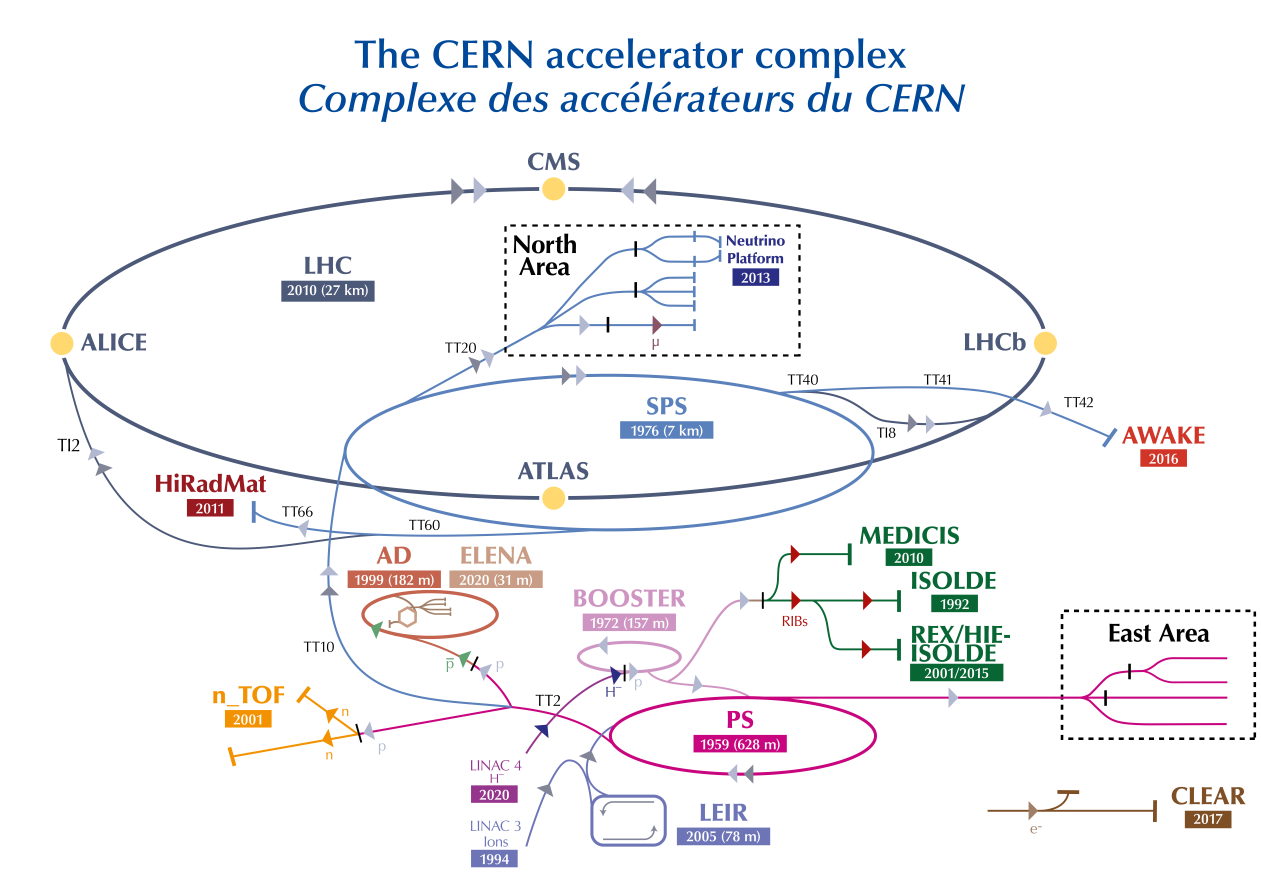
\includegraphics[width=1\textwidth]{cap1/acceleratori_CERN}
	\caption{Schema del complesso di acceleratori del CERN}
	\label{fig:acceleratori_cern}
\end{figure}

Alla data odierna il complesso del CERN è costituito da nove acceleratori (e due deceleratori): ognuno di questi accelera le particelle a energie sempre più elevate per poi passare mano a mano ad acceleratori sempre più grandi.
Attualmente LHC (\textit{Large Hadron\footnote{Gli adroni sono particelle subatomiche composte; i più comunemente conosciuti sono i neutroni e i protoni.} Collider}) è l'acceleratore di particelle più potente e grande del mondo: installato nel 2008, fa collidere fasci di protoni a velocità vicine a quella della luce per studiare le particelle fondamentali.
Si trova in un tunnel posto a 100 metri di profondità ed è costituito da un anello lungo 27 chilometri di magneti superconduttori mantenuti a una temperatura di $‑271.3 \degree C$ \cite{CERN_LHC}.

% ====================================================
%
% I NEUTRINI
%
% ====================================================
\section{I Neutrini}
I leptoni sono una famiglia di particelle elementari appartenenti alla classe dei fermioni.
Si dividono in tre generazioni, ciascuna composta da una particella carica e dal rispettivo neutrino associato: l'elettrone ($e$), il muone ($\mu$) e il tau ($\tau$).

Il neutrino è una particella subatomica elementare di massa piccolissima (non ancora precisamente determinata) e carica elettrica nulla che interagisce molto raramente con la materia, tanto che la stessa Terra è praticamente trasparente per essi.
L’ipotesi dell’esistenza dei neutrini fu formulata inizialmente da W. Pauli nel 1930; tuttavia, a causa della loro particolare elusività, furono rilevati per la prima volta solamente nel 1956 in un esperimento condotto da C. Cowan e F. Reines in un reattore nucleare negli Stati Uniti.
A questo seguirono scoperte sui neutrini che andarono ad arricchire il panorama della fisica delle particelle, portando alla scoperta di tre famiglie --- dette sapori --- di neutrini: elettronico, muonico e tau, ciascuno associato univocamente al rispettivo leptone carico e indicato con i simboli $\nu_e$, $\nu_\mu$ e $\nu_\tau$.

\begin{figure}[H]
	\centering{}
	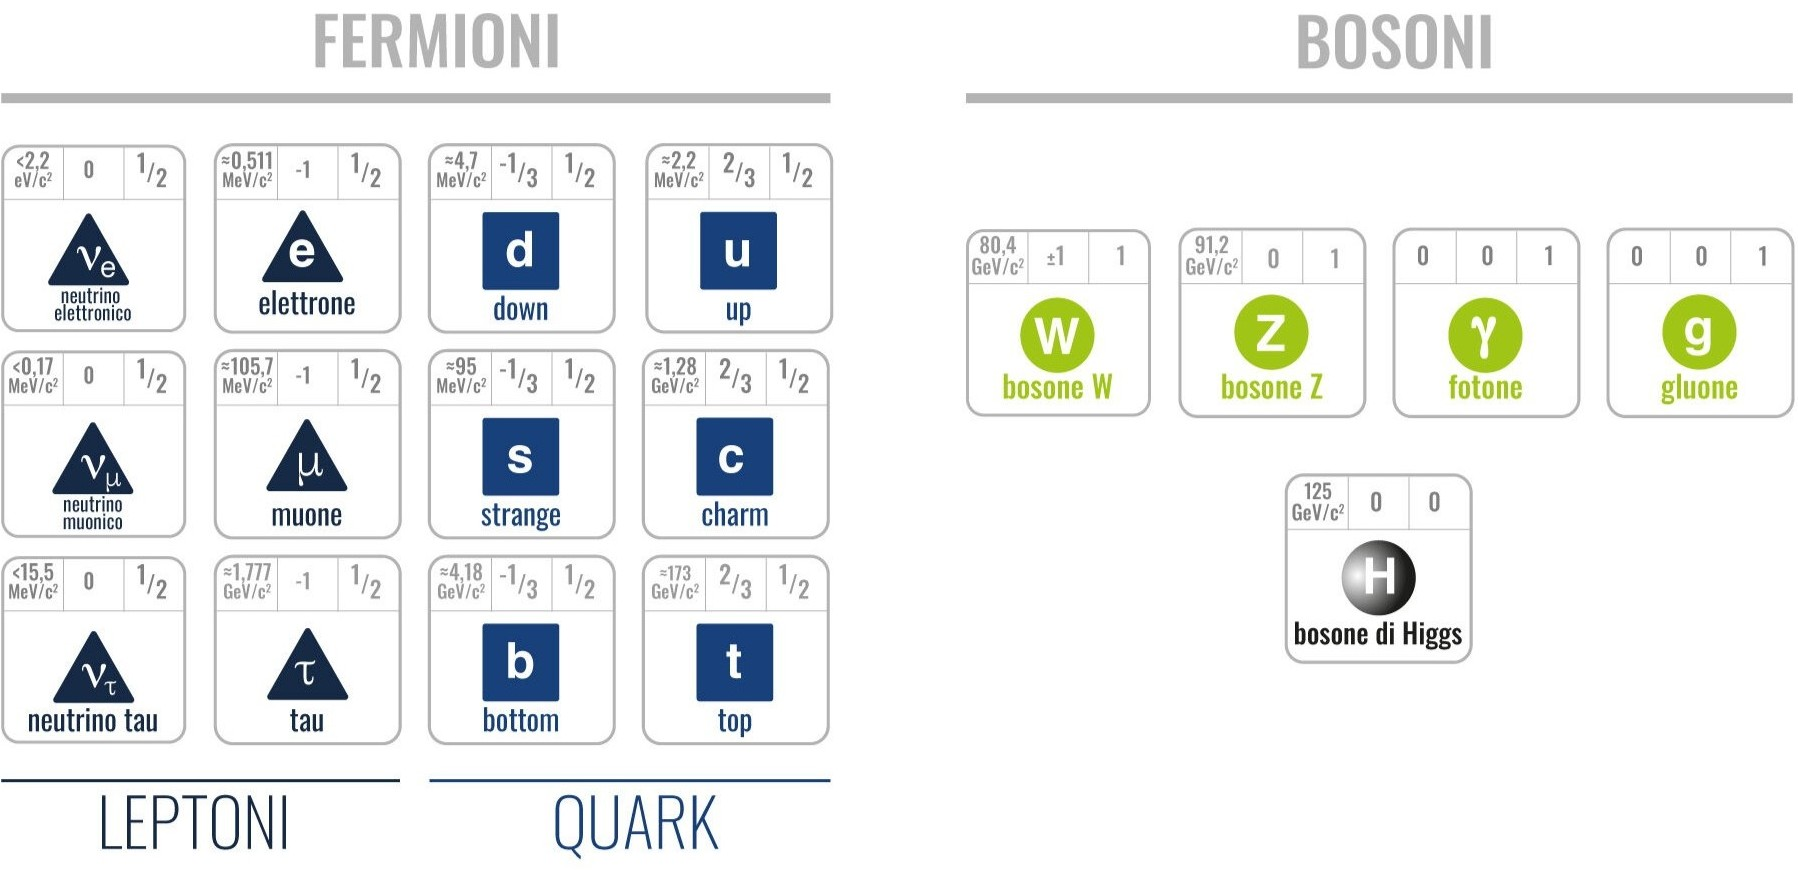
\includegraphics[width=0.97\textwidth]{cap1/modello_standard_infn}
	\caption[Particelle elementari del Modello Standard]{Particelle elementari del Modello Standard (\copyright~INFN)}
\end{figure}

I tre tipi di neutrino sono soggetti ad un fenomeno chiamato oscillazioni di sapore per cui, in certe condizioni, si possono trasformare l’uno nell’altro: l’esistenza di questo fenomeno implica che i neutrini debbano avere una massa, seppur piccolissima, diversa tra loro.
Questo risultato è in disaccordo con il Modello Standard che, al contrario, prevede che i neutrini abbiano massa nulla \cite{lngs_neutrini}.

% ====================================================
%
% OBIETTIVI
%
% ====================================================
\section{Obiettivi}
Negli scorsi decenni le misure della sezione d’urto nelle interazioni di neutrino sono state per lo più effettuate a basse energie (al di sotto di 350 GeV): la regione tra i 350 GeV e i 10 TeV è rimasta sconosciuta fino a qualche anno fa \cite{Bustamante_Connolly}.
I neutrini prodotti ad LHC consentono di osservarne le interazioni in un range di energie mai studiato che va da qualche centinaio di GeV a poche decine di TeV.
L’alta intensità delle collisioni protone-protone si traduce in un abbondante flusso di neutrini, e le alte energie dei neutrini prodotti implicano sezioni d’urto relativamente grandi \cite{SND_Observation}.

La sua posizione leggermente fuori asse rispetto alla linea di collisione dei fasci di protoni di LHC fa sì che l'intervallo di pseudorapidità\footnote{In fisica delle particelle, la pseudorapidità è una coordinata spaziale usata per descrivere l'angolo relativo tra una particella e l'asse del fascio.} dei neutrini studiati cada in una regione precedentemente inesplorata \cite{LHCb_Charm}.
Per questa caratteristica SND si differenzia dall'esperimento FASER (\textit{ForwArd Search ExpeRiment}), che è invece posizionato sulla traiettoria del fascio.

L'esistenza di queste particelle rappresenta quindi una prova dell’esistenza di una fisica che va oltre il Modello Standard \cite{Marfatia_2015}, e analizzandone le caratteristiche potremo avere un nuovo punto di vista per studiare l'universo \cite{Ackermann_2019}.

% ====================================================
%
% UBICAZIONE DELL'ESPERIMENTO
%
% ====================================================
\section{Ubicazione dell'esperimento}
TI18 è un tunnel lungo 280m che si innesta nell'anello di LHC tramite il punto di giunzione UJ18, a circa 480 m dal punto di impatto di ATLAS\footnote{ATLAS (\textit{A Toroidal LHC ApparatuS}) è uno dei nove rivelatori di particelle costruiti per LHC installato nel 2008.} (vedi posizione in \cref{fig:acceleratori_cern}).
Era stato inizialmente costruito per l’iniezione di positroni\footnote{Il positrone, chiamato anche antielettrone, è l'antiparticella dell'elettrone: rispetto a quest'ultimo, ha la stessa massa ma carica elettrica uguale e opposta.} dall’SPS (\textit{Super Proton Synchrotron}) all’acceleratore LEP (\textit{Large Electron-Positron Collider}), quest'ultimo rimosso alla fine del 2000 per cedere il posto ad LHC, ponendo così in disuso TI18.

\begin{figure}[H]
	\centering{}
	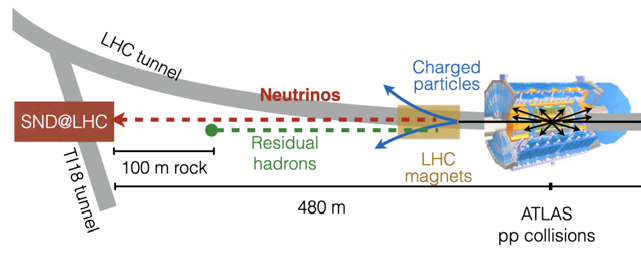
\includegraphics[width=0.9\textwidth]{cap1/posizione_snd}
	\caption[Posizione del rivelatore SND@LHC]{Posizione del rivelatore SND@LHC: a sinistra il tunnel TI18 in cui è collocato SND, a destra il punto di collisione IP1 di ATLAS}
\end{figure}

Il tunnel TI18 è stato successivamente chiuso, ad eccezione di una piccola sezione di circa 20m prima di entrare nella giunzione UJ18 con LHC.
Questa collocazione risulta particolarmente adeguata dal momento che il breve tratto scelto intercetta l’asse di collisione di IP1\footnote{L'IP1 (\textit{Interaction Point 1}) identifica il punto di interazione in cui avvengono le collisioni tra i fasci di protoni di LHC all'interno dell'esperimento ATLAS.}.
Poiché l’esperimento SND@LHC si propone di sondare una regione di alta pseudorapidità (ricordiamo che è l’angolo relativo tra una particella e l’asse del fascio), il rivelatore è stato posizionato leggermente fuori asse.

\begin{figure}[H]
	\centering{}
	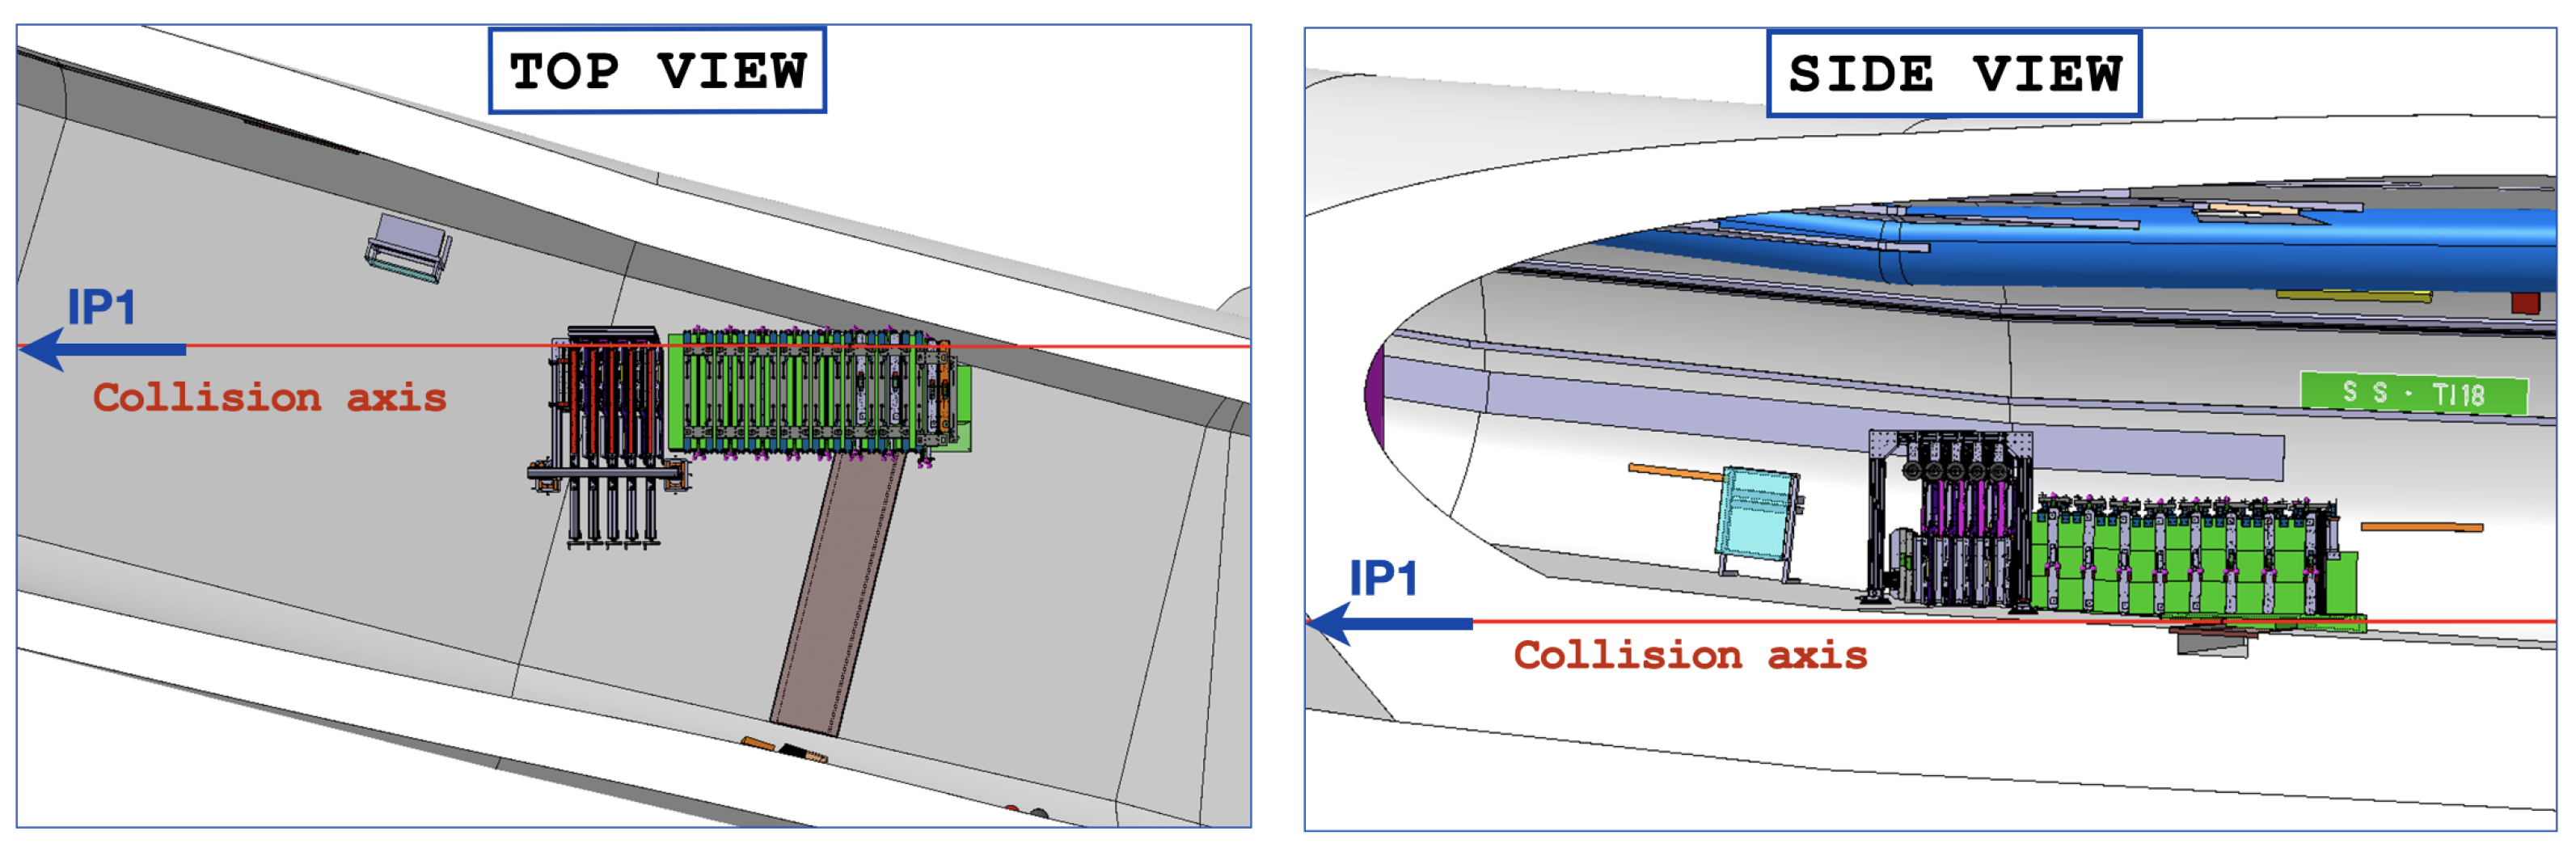
\includegraphics[width=1\textwidth]{cap1/asse_IP1}
	\caption{Vista laterale e dall’alto del rivelatore nel tunnel TI18}
\end{figure}

% ====================================================
%
% STRUTTURA DEL RIVELATORE
%
% ====================================================
\section{Struttura del rivelatore}
La struttura di SND@LHC è stata studiata per far sì che possano essere identificati tutti e tre i sapori di neutrino sfruttando lo spazio a disposizione nel tunnel TI18.
Grazie all'esperimento OPERA\footnote{OPERA è stato un esperimento (2008 - 2012) posizionato ai Laboratori Nazionali del Gran Sasso per lo studio dell'oscillazione di sapore dei neutrini muonici in neutrini tau.} è stato dimostrato che la soluzione ottimale è data dalla combinazione di emulsioni nucleari e rivelatori elettronici \cite{R_Acquafredda_2009}.

\begin{figure}[H]
	\centering{}
	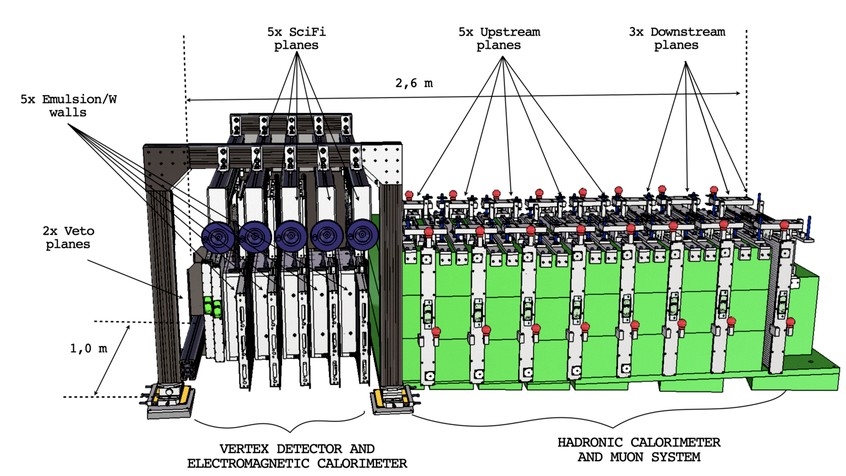
\includegraphics[width=1\textwidth]{cap1/rivelatore}
	\caption{Struttura dell’esperimento SND@LHC}
	\label{fig:rivelatore}
\end{figure}

Attualmente il rivelatore è composto dai seguenti sistemi (da sinistra a destra in \cref{fig:rivelatore}):
\begin{itemize}
	\item Sistema di veto: scherma il rivelatore dalle particelle cariche (principalmente muoni di LHC) che entrano frontalmente, permettendo di discriminare i prodotti delle interazioni neutre.
	\item Volume bersaglio: composto da pareti di emulsioni nucleari alternate a piani di tracciatori elettronici (SciFi), funge da rivelatore di vertice e fornisce la marcatura temporale agli eventi ricostruiti nelle emulsioni. Nella vista frontale di \cref{fig:schema_struttura} viene messa in evidenza la regione di pseudorapidità $7.2 < \eta < 8.4$.
	\item Sistema di identificazione dei muoni: situato a valle del bersaglio, identifica i muoni e agisce come calorimetro adronico\footnote{Un calorimetro adronico (HCAL, \textit{Hadronic Calorimeter}) è uno strumento progettato per misurare l'energia degli adroni.} campionato per la misura dell'energia degli sciami.
\end{itemize}

\begin{figure}[H]
	\centering{}
	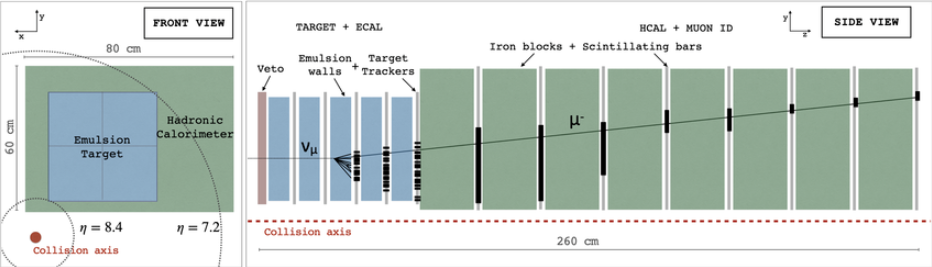
\includegraphics[width=1\textwidth]{cap1/struttura}
	\caption[Viste schematiche della struttura]{Rappresentazione schematica della vista frontale (sinistra) e laterale (destra) del rivelatore}
	\label{fig:schema_struttura}
\end{figure}

% ====================================================
% VETO
% ====================================================
\subsection{Veto}
Il sistema di veto è necessario per riconoscere le particelle cariche rilevate da SND provenienti frontalmente dall'esterno.
Questo filtro è indispensabile poiché si vogliono studiare gli eventi in cui vengono prodotte delle particelle cariche a partire dall'interazione di particelle neutre (ad esempio un neutrino muonico $\nu_\mu$ che urtando un nucleo di tungsteno si trasforma in un muone $\mu^{-}$): se entra una particella già carica, l'evento non è rilevante ai fini dello studio.

Alla base del suo funzionamento vi sono le barre scintillanti (SciFi, \textit{Scintillating Fibre}), ovvero delle barre che emettono scintille luminose al passaggio di particelle cariche, che vengono poi lette da fotosensori posti alle loro estremità.
Il sistema è composto da due piani paralleli di barre, ognuna delle quali ha dimensioni $42 \times 6 \times 1\,\text{cm}^3$ ed è avvolta in un foglio di alluminio
per assicurare l’opacità e isolarla dalla luce proveniente da barre adiacenti.
Ciascun piano comprende sette barre scintillanti racchiuse in una struttura di alluminio con pareti dello spessore di $4\,\text{mm}$.
Ogni estremità di ciascuna barra è letta da otto fotosensori a silicio (SiPM, \textit{Silicon Photomultiplier}), che convertono i segnali luminosi in impulsi elettrici.
Lo scostamento verticale di 2cm tra i due piani, consente di ottenere la massima copertura del bersaglio nonostante la presenza di spazi tra le barre indotti dalle variazioni delle loro altezze ($\sim250\,\mu\text{m}$) e dai fogli di alluminio ($\sim60\,\mu\text{m}$) \cite{Acampora_2024}.

% ====================================================
% BERSAGLIO E RIVELATORE DI VERTICE
% ====================================================
\subsection{Bersaglio e rivelatore di vertice}
Il bersaglio di SND@LHC è la sezione del rivelatore dove avvengono effettivamente le interazioni dei neutrini: è stato progettato in maniera tale da essere allo stesso tempo sia una massa in cui far avvenire le interazioni, sia un rivelatore ad altissima precisione.
Il vertice è infatti il punto esatto in cui il neutrino interagisce con un altro nucleo (nel nostro caso il tungsteno), trasformandosi poi in altre particelle: è necessaria una risoluzione spaziale estrema per identificare questo punto.

Strutturalmente, è composto da cinque muri di sezione trasversale $384 \times 384 \,\text{mm}^2$ a loro volta divisi in quattro celle elementari dette mattoni. Ogni mattone è costruito sulla base della tecnologia ECC (\textit{Emulsion Cloud Chambers}): 60 film di emulsioni nucleari (ognuno spesso $300\,\mu\text{m}$ e di sezione trasversale $192 \times 192 \,\text{mm}^2$) usati come dispositivi di tracciamento sono intervallati a 59 piatti di tungsteno spessi $1 \,\text{mm}$ che fungono da bersaglio per i neutrini.
Il mattone risultante (rappresentato in \cref{fig:muro_bersaglio}) ha uno spessore totale di circa $78\,\text{mm}$ e una massa di $41.5\,\text{kg}$, facendo sì che la massa totale del bersaglio composto dai cinque muri di $2\times2$ mattoni sia di $830\,\text{kg}$. A ogni muro del bersaglio è intervallato un piano di fibre scintillanti (SciFi) \cite{Acampora_2024}.

\begin{figure}[H]
	\centering{}
	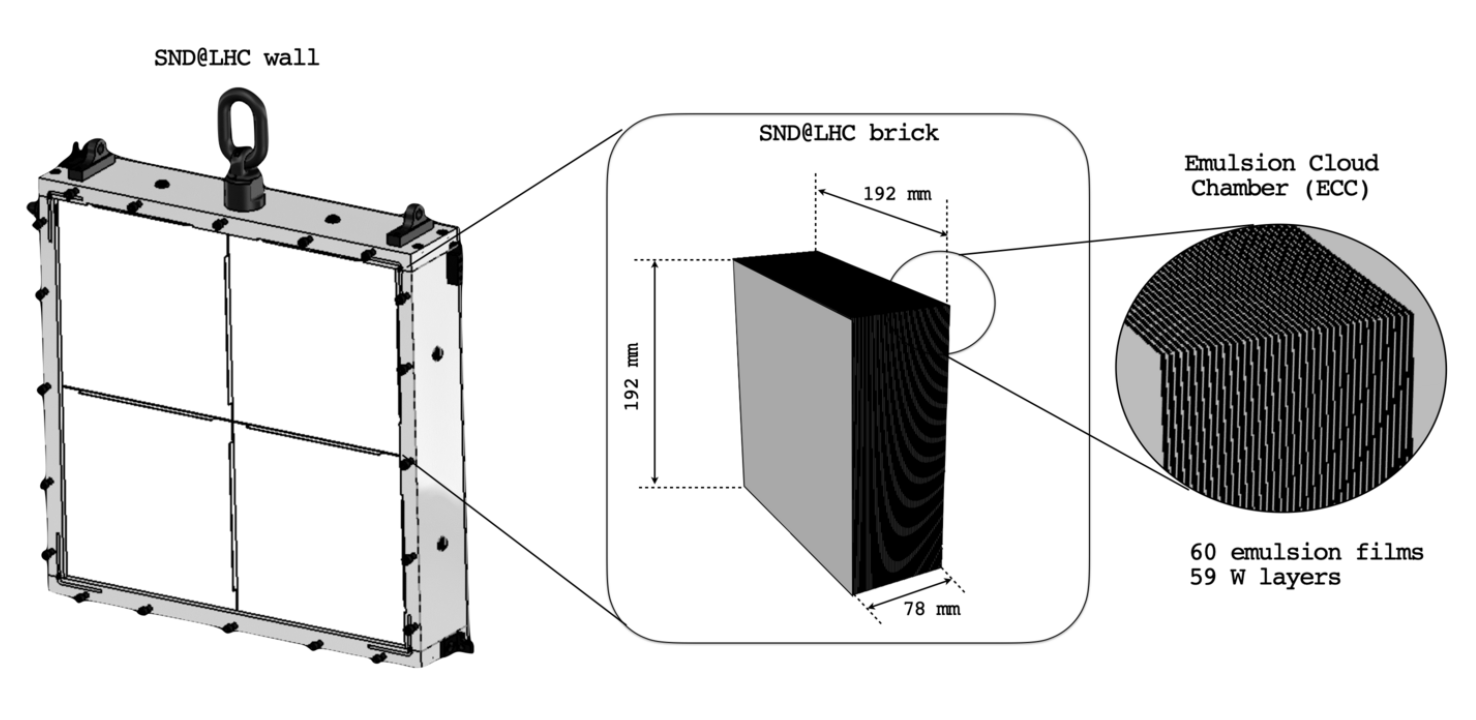
\includegraphics[width=1\textwidth]{cap1/muro_bersaglio}
	\caption[Dettaglio di una parete del bersaglio]{Una parete a emulsione è composta da quattro mattoni, ciascuno costituito da 60 pellicole di emulsione intervallate da 59 fogli di tungsteno}
	\label{fig:muro_bersaglio}
\end{figure}

\subsubsection{Emulsioni}
I film di emulsioni nucleari sono il rivelatore tridimensionale più leggero e compatto che garantisce al contempo una risoluzione spaziale submicrometrica e angolare al milliradiante. Durante lo sviluppo dei film in camera oscura è utilizzato un processo chimico che permette di ottenere dei cluster dal diametro di $0.6\,\mu\text{m}$ della traccia lasciata dalle particelle cariche che li hanno attraversati.

Un film è composto da due strati dallo spessore di $70\,\mu\text{m}$ separati da una base plastica trasparente di $170\,\mu\text{m}$.
Nel rivelatore sono impiegati 1200 film di emulsioni, per un totale di $44\,\text{m}^2$ analizzati da microscopi ottici completamente automatizzati a un ritmo di $\sim180\,\text{cm}^2\text{/h}$.

Collegando i punti rappresentanti il passaggio di una particella carica su entrambi gli strati del film è possibile misurare la direzione angolare della traccia, permettendo di distinguere i tre diversi sapori di neutrino.

\begin{figure}[H]
     \centering
     \begin{subfigure}[b]{0.32\textwidth}
         \centering
         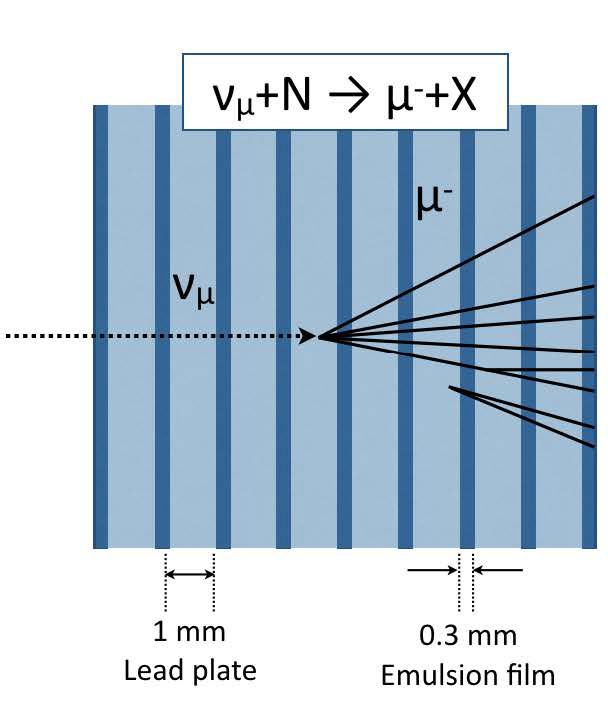
\includegraphics[width=\textwidth]{cap1/scattering_emulsioni_muonico}
         \caption{Neutrino muonico}
     \end{subfigure}
     \hfill
     \begin{subfigure}[b]{0.32\textwidth}
         \centering
         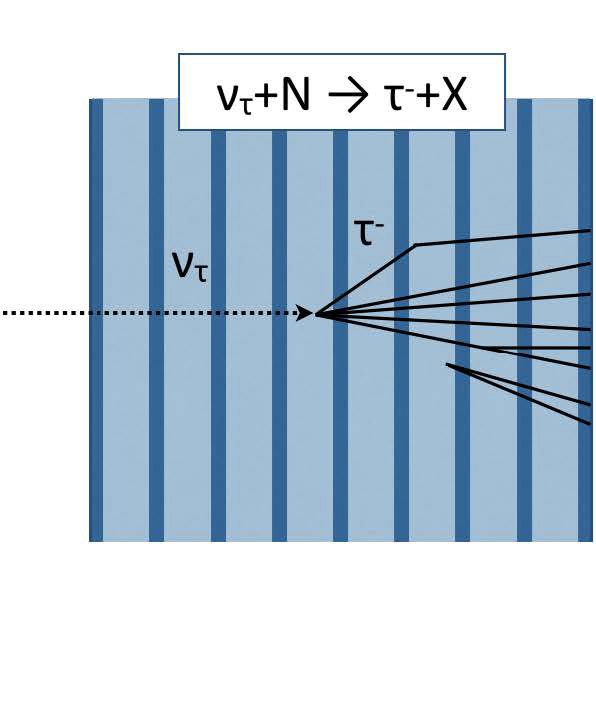
\includegraphics[width=\textwidth]{cap1/scattering_emulsioni_tau}
         \caption{Neutrino tau}
     \end{subfigure}
     \hfill
     \begin{subfigure}[b]{0.32\textwidth}
         \centering
         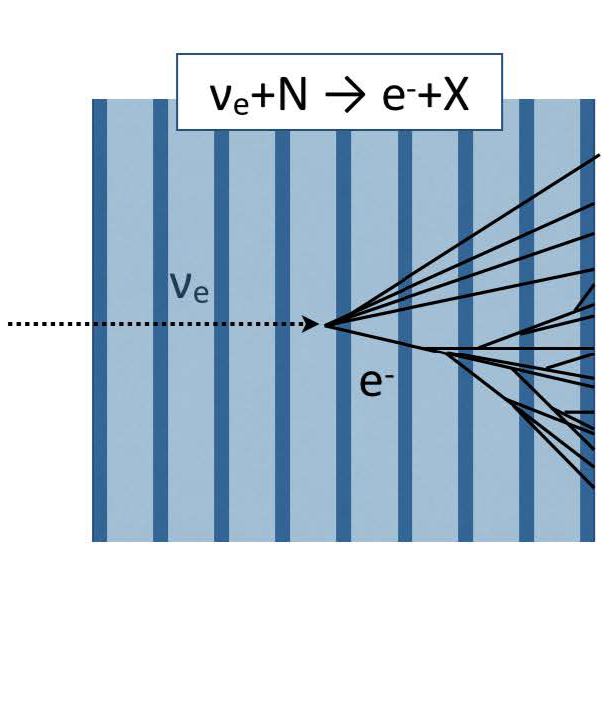
\includegraphics[width=\textwidth]{cap1/scattering_emulsioni_elettronico}
         \caption{Neutrino elettronico}
     \end{subfigure}
        \caption[Tracce dei tre sapori di neutrino nei film di emulsioni]{Schematizzazione dello scattering dei tre sapori di neutrino nelle pareti di emulsioni}
\end{figure}

\subsubsection{Piani SciFi}
I cinque piani di fibre scintillanti, alternati agli altrettanti di muri del bersaglio, costituiscono il sistema di tracciamento di SND.
Ogni piano è costituito da 6 strati di fibre dal diametro di $250\,\mu\text{m}$, offrendo una risoluzione spaziale di $\sim50\,\mu\text{m}$ e temporale di $\sim250\,\text{ps}$.
\begin{figure}[H]
	\centering{}
	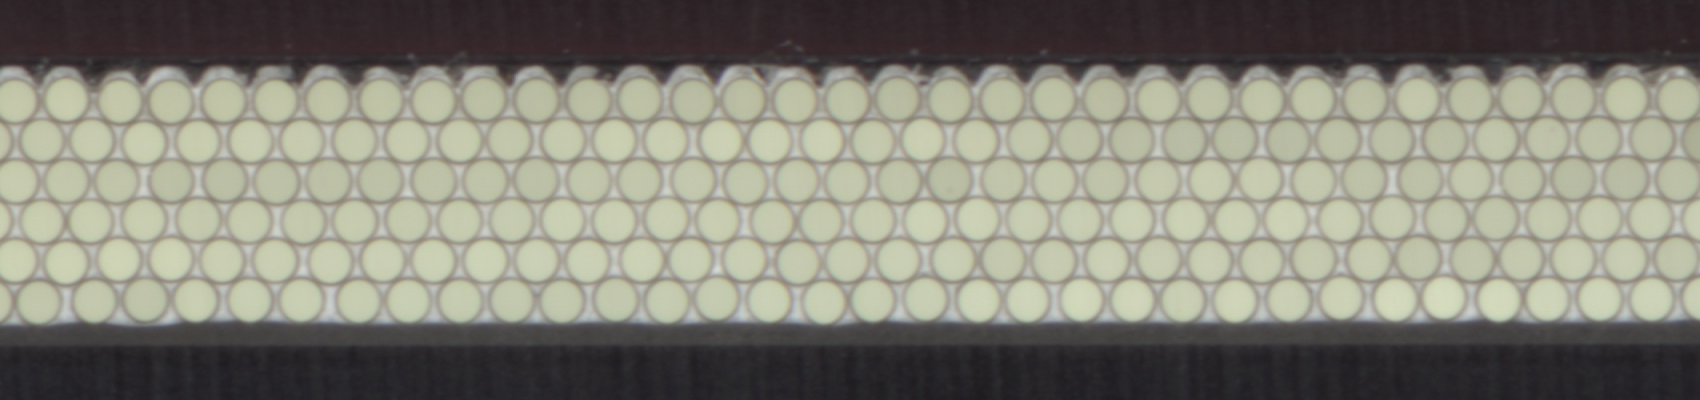
\includegraphics[width=0.5\textwidth]{cap1/fibre_scifi}
	\caption[Fibre che compongono il piano SciFi]{Dettaglio dei sei strati di fibre che compongono un piano SciFi}
\end{figure}
Poiché le emulsioni nucleari rimangono a raccogliere dati per svariato tempo, tramite le rilevazioni elettroniche delle scintille in SciFi è possibile assegnare un tempo preciso alle interazioni di neutrino impresse nei film.
Inoltre, permettono anche di misurare l'energia degli sciami elettromagnetici e adronici prodotti in tali interazioni.

% ====================================================
% SISTEMA DI IDENTIFICAZIONE DEI MUONI
% ====================================================
\subsection{Sistema di identificazione dei muoni}
A valle del bersaglio di SND@LHC è presente il sistema di rilevazione di muoni.
Il suo scopo principale è quello di identificare i muoni e, insieme alle SciFi, costituisce anche un calorimetro adronico per la misura dell’energia degli sciami adronici.

È composto da 8 strati di piani scintillanti, alternati a blocchi di ferro spessi 20cm che fungono da materiale passivo.
Se una particella attraversa tutti gli otto piani è quasi sicuramente identificata come un muone: interagendo poco con la materia, essi possono penetrare quasi indisturbati gli strati del rivelatore.

Il sistema è diviso in due regioni: i primi cinque piani a monte (\textit{upstream}, US) e gli ultimi tre a valle (\textit{downstream}, DS), serviti rispettivamente da tre e due DAQ (\textit{Data Acquisition System}) \cite{Acampora_2024}.

\begin{figure}[H]
	\centering{}
	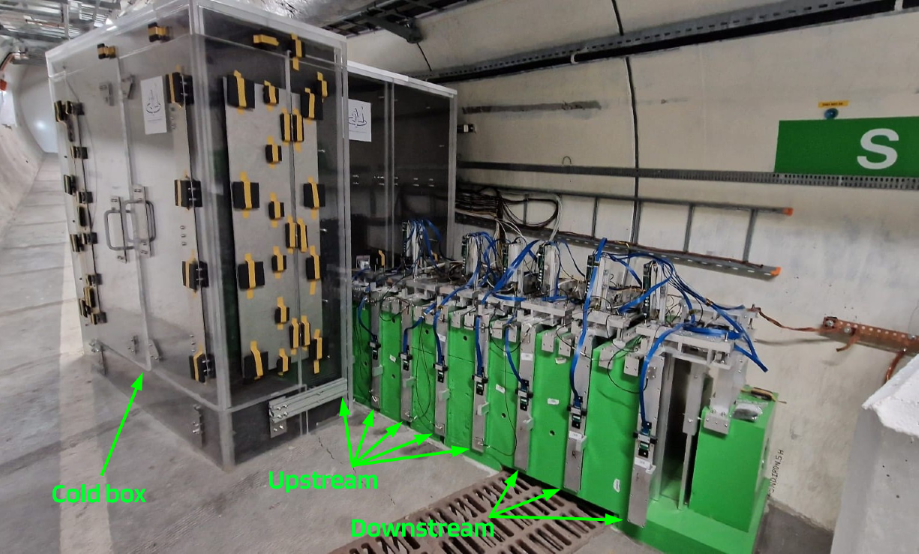
\includegraphics[width=0.75\textwidth]{cap1/sistema_muoni}
	\caption[Foto del sistema di identificazione di muoni]{Foto del sistema di identificazione dei muoni, in cui vengono messi in evidenza le due regioni US e DS, e i DAQ}
\end{figure}

\subsubsection{Upstream - US}
I 5 piani di US sono simili ai piani del sistema di veto, ad eccezione delle dimensioni.
Ogni piano è formato da 10 barre scintillanti sovrapposte, ognuna di dimensioni $1 \times 6 \times 83 \,\text{cm}^3$, ricomprendo un'area di $81 \times 60 \,\text{cm}^2$. Così come accade per quelle del sistema di veto, ogni barra è avvolta in un foglio di alluminio e ognuna delle sue estremità è letta da otto SiPM.

\subsubsection{Downstream - DS}
Gli ultimi tre piani completano l'identificazione dei muoni: essendo caratterizzati da un’alta granularità, la regione DS consente di determinarne la posizione con una risoluzione migliore.
Ogni piano è formato da due strati di barre scintillanti: il primo strato è composto da 60 barre orizzontali da $1 \times 1 \times 82.5 \,\text{cm}^3$, il secondo da 60 barre verticali da $1 \times 1 \times 63.5 \,\text{cm}^3$.
Ogni barra orizzontale è letta da un SiMP a ogni estremità; quelle verticali sono lette da un solo SiPM all’estremità superiore.
Anche in questo caso le barre sono avvolte strettamente da fogli di alluminio per minimizzare la perdita di luce a causa di riflessioni multiple.
Per le barre verticali, all’estremità inferiore non collegata ad alcun SiMP, vi è un altro strato piatto che ottimizza la riflessione.

\begin{figure}[H]
     \centering
     \begin{subfigure}[b]{1\textwidth}
         \centering
         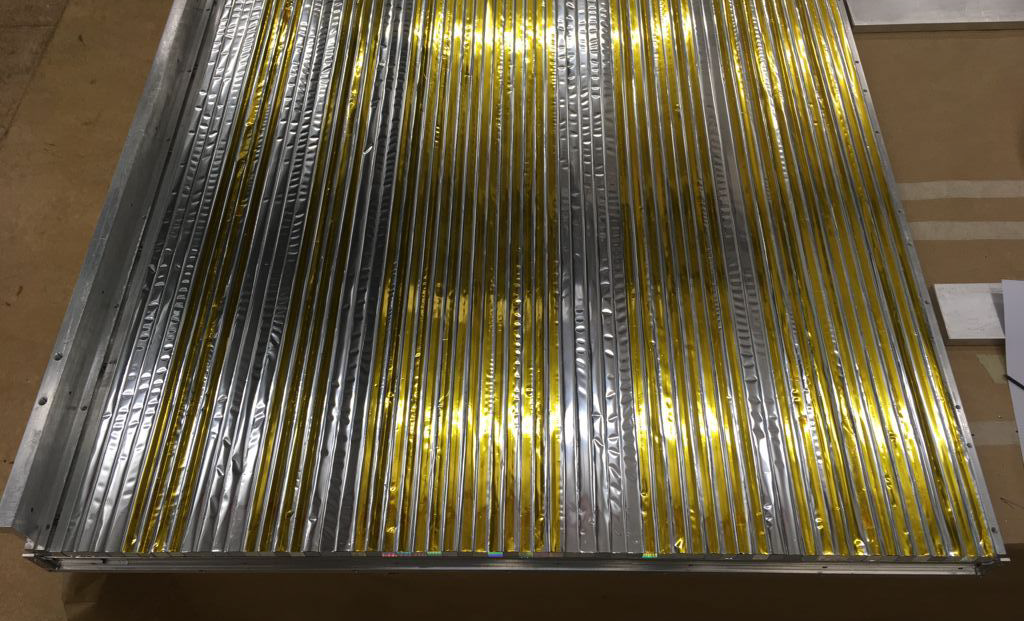
\includegraphics[width=\textwidth]{cap1/foto_scifi}
         \caption{60 barre SciFi}
     \end{subfigure}
     \hfill
     \begin{subfigure}[b]{1\textwidth}
         \centering
         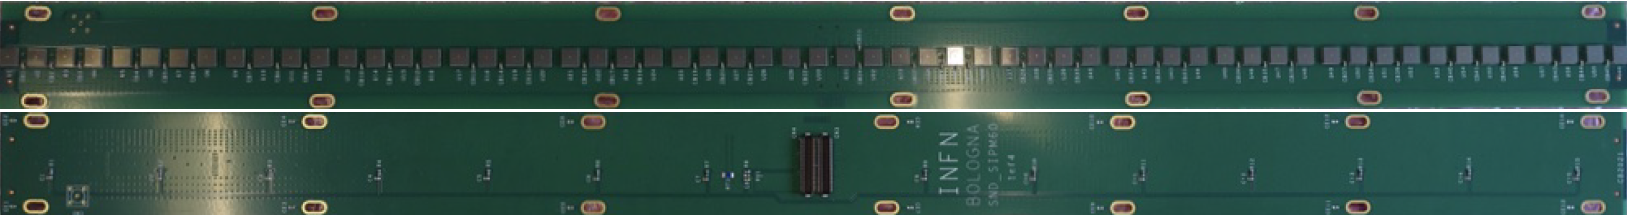
\includegraphics[width=\textwidth]{cap1/pcb_sipm}
         \caption{PCB su cui alloggiano i SiPM delle SciFi}
     \end{subfigure}
        \caption[Foto dei componenti di un piano SciFi di DS]{Foto scattate durante il processo di produzione di un piano SciFi di DS}
\end{figure}
\chapter*{Conclusioni}
\addcontentsline{toc}{chapter}{Conclusioni}
Testo conclusivo.


% ====================================================
%
% BIBLIOGRAFIA
%
% ====================================================
\cleardoublepage % Chiude il capitolo precedente
\phantomsection % Crea l'ancora per hyperref
\addcontentsline{toc}{chapter}{Bibliografia}
\markboth{BIBLIOGRAFIA}{BIBLIOGRAFIA} % Aggiorna l'intestazione della pagina
\bibliographystyle{ieeetr}
\bibliography{resources/bib/Bibliografia}


% ====================================================
%
% RINGRAZIAMENTI
%
% ====================================================
\cleardoublepage
\chapter*{Ringraziamenti}
\pagestyle{empty}
\thispagestyle{empty}

Desidero innanzitutto ringraziare la mia relatrice, la prof.ssa Damiana Lazzaro, per avermi seguito con enorme costanza e dedizione durante i corsi da lei tenuti e per tutta la durata del tirocinio e della stesura della tesi.
Il supporto dato è stato fondamentale per produrre questo elaborato, unito a un sostegno umano sempre presente.
È inoltre riuscita a trasmettermi la sua passione per la matematica, utilizzata come strumento per comprendere a fondo le cose, e non come mezzo di tortura verso i suoi studenti.

Un pensiero importante va anche ai miei correlatori, il prof. Luigi Guiducci e la dott.ssa Giulia Paggi, e al resto del gruppo dell'INFN di Bologna, il dott. Filippo Mei e la dott.ssa Licia Mozzina.
Mi avete guidato con grande pazienza passo dopo passo all'interno del software di SND con supporto costante, dedicandomi molto tempo sebbene scarso per voi in primis.
Avete inoltre fatto di tutto per regalarmi l'esperienza indimenticabile vissuta al CERN tutti insieme: credo non ci siano parole per descrivere quanto accaduto in quei fantastici giorni, tra colpi di uncinetto nella sala conferenze e qualche birra ai barbecue.
Per tutti quelli che non erano presenti, giuro che ci sono stati anche dei momenti seri.

Un grazie di cuore ai miei genitori e ai miei fratelli, per tutto ciò che avete fatto per me in questi anni: senza il vostro supporto e incoraggiamento non sarei qui oggi.
A mia mamma Erica per comprendere le mie difficoltà e a mio padre Andrea per gli sproni continui.
A mio fratello Matteo, per essere anche il mio migliore amico, e a mia sorella Matilde, per voler stare con me fino all'ultimo minuto prima di tornare a Cesena.
Sappiate che questo traguardo è anche vostro.

\needspace{3\baselineskip}
Grazie a te, Ale, tu che mi hai supportato soprattutto in questo ultimo duro anno, tra un piantino di sfogo e un episodio di Stranger Things.
A furia di parlare di università, ormai conosci i nomi dei miei professori meglio di me; hai sopportato in prima persona ogni mio alto e basso di questo percorso, consolandomi quando ne avevo bisogno.
Ti ringrazio anche per il supporto che mi dai persino nelle piccole cose; forse gli invitati alla festa devono ringraziarti se siamo riusciti ad organizzare qualcosa oggi.

Come potrei non citarti, Gianluca: abbiamo iniziato il nostro percorso insieme nel 2018, quando ancora non sapevamo cosa fosse un'equazione (non posso dire un ciclo for, visto che tu eri già avanti).
Benché le nostre strade si siano separate, ci siamo comunque ritrovati ad aggiornarci tutti i giorni sui corsi che stavamo affrontando.
Con Emily, ci siamo tuffati a capofitto nel mondo dell'università, passando intere giornate immersi tra gli orientamenti e gli esercizi dei test d'ingresso.
Si potrebbe quasi dire che le mie scelte sono anche un po' colpa vostra (o merito, a seconda dei punti di vista).
Sappiate che mi dispiace per tutte le volte che, assieme ad Ale, Vincenzo, Viola, Giuseppe e Tommaso, vi ho tartassati di messaggi sul mio percorso universitario; credo che a questo punto sareste in grado di discutere la tesi al mio posto.

A Mattia, che è ormai il mio compagno di viaggio da quasi venti anni.
E lo intendo letteralmente, dai viaggi in bicicletta a quelli sull'Intercity 614 per ritornare alla realtà di tutti i giorni dopo il weekend passato a casa.
Se in questi anni mi sono trasformato, lo devo anche al tuo incoraggiamento, insieme a quello di David, Sheron e Martina.

I miei due più stretti unifriend, che a farlo apposta non ci sarei riuscito, sono Nicolas e Nicholas, aka Nico e Svitol.
Abbiamo affrontato fianco a fianco qualsiasi difficoltà, partendo dal primo esercizio di analisi fino ad arrivare all'ultimo progetto di gruppo; e di progetti ne abbiamo dovuti fare eh.
Senza di voi (e le piadinate fatte alla piadineria Irma) la laurea non avrebbe avuto lo stesso senso.

A Giulio, Lorenzo e Matteo -- ordine rigorosamente alfabetico per non far torto a nessuno --, con cui in questo anno da fuorisede abbiamo condiviso di tutto: piatti per la cena, sedie di casa orripilanti, notti passate a ripassare prima degli esami e chi più ne ha più ne metta.
Avete reso la lontananza da casa un peso molto più gestibile di quello che sarebbe stato senza di voi.

Un bacio va a voi nonni -- Duilio, Assunta, Eliseo e Lilliana -- per avermi sempre voluto bene, nutrito (forse un po' troppo) e sostenuto da quando ancora non sapevo camminare.

Anche voi, zii e cugini, ad ogni esame mi avete sempre chiesto come fosse andata e, nonostante la lontananza o gli impegni personali, siete sempre riusciti a trovare un modo per scambiare due chiacchiere.
Capite anche voi però che elencarvi tutti richiederebbe una tesi a parte!

Grazie infine a tutti voi che, sebbene non nominati nelle righe precedenti, mi siete stati accanto in tutti questi anni e state ora leggendo queste parole, o ascoltando se sarò in grado di recitarvele, ma direi che arrivati a questo punto la risposta si saprà già.

Vorrei dedicare un ultimo pensiero a me stesso, per aver sempre tenuto duro anche quando le cose hanno iniziato a farsi difficili; ma alla fine, mio padre mi ha sempre detto che quando il gioco si fa duro, i duri iniziano a giocare.

Finalmente lo possiamo dire, anche a chi non ci contava:\\
\#ciVediamoAllaLaurea.

\end{document}